\documentclass[conference]{IEEEtran}
\IEEEoverridecommandlockouts
% The preceding line is only needed to identify funding in the first footnote. If that is unneeded, please comment it out.
\usepackage{cite}
\usepackage{amsmath,amssymb,amsfonts}
\usepackage{algorithmic}
\usepackage{graphicx}
\usepackage{textcomp}
\usepackage{xcolor}
\def\BibTeX{{\rm B\kern-.05em{\sc i\kern-.025em b}\kern-.08em
T\kern-.1667em\lower.7ex\hbox{E}\kern-.125emX}}
\begin{document}

    \title{Vehicle Accident Prevention System at Hairpin Bends\\{
    \large Using IR Sensors and Arduino
    }

        }

    \author{\IEEEauthorblockN{ Kedar Salunkhe}
    \IEEEauthorblockA{
    Roll no. C54 \\
    PRN no. 2122000465}
    \and
    \IEEEauthorblockN{Sandip Sannake}
    \IEEEauthorblockA{
    Roll no. C59 \\
    PRN no. 2122000621}
    \and
    \IEEEauthorblockN{Abhijit Shende}
    \IEEEauthorblockA{
    Roll no. C63 \\
    PRN no. 2122000659}
    \and
    \IEEEauthorblockN{Tejas Chavan}
    \IEEEauthorblockA{
    Roll no. C70 \\
    PRN no. 2122000357}
    \and
    \IEEEauthorblockN{Digvijay Patil}
    \IEEEauthorblockA{
    Roll no. 71 \\
    PRN no. 2122000814}

    }

    \maketitle

    \begin{abstract}
        In the developing countries there are many dangerous roads where accidents and causes very lethal effects now a day.
        If we talk about dangerous roads in the world then all of them are mountain roads, T roads, narrow roads. Some mountain
        roads are narrow, having many curves and very tight, this cause of the most hazards.
        Vehicle accident prevention system can be crucial step in accident safety on hilly and mountain roads. We have recognized our
        past, thousands of accidents and death on mountain road, some even fall of the cliff and after that can not view even be traced.
        Such accidents not only destroy human life but also major loss financially to the individual and government also. To avoid such
        problems in curve roads mountain areas, we have proposed this vehicle accident prevention system. The main objective of this
        model is to diminish the accident in hairpin bends an U turnings.Sometimes it observes that the vehicle driver unable to see the
        vehicle reaching form opposite side due to lack of vision and the serious accidents are happened. Though this type of project
        ideas can help to decrease these type of problems.
    \end{abstract}

    \begin{IEEEkeywords}
        Arduino , Cables , Connector , IR Sensors , Buzzers , Power Supply , PCB Breadboards , Hairpin Bends.
    \end{IEEEkeywords}

    \section{Problem Definition}
    According to million death study (MDS) about 2.3 million people die in India per year. In that 137K is because of road accidents.
    That about 377 peoples per day. In that 3.7\% are because of unexpected obstacles.There are many risky roads and bends in the world
    like mountain roads, narrow curve roads and hair pin bends for ex. Kolli hill roads, Gata Loops,3-Level Zig-zag roads in Sikkim,
    Leh Manali Highway.
    The problem in the hair pin bends is that the drivers are unable to see the vehicle or obstacles coming from opposite side of the
    curve. If the vehicle is in high speed, then it is difficult to control the speed of the vehicle and there are chances of falling to a cliff
    and sometimes people not get traced. Not only accident is common thing for this type of places but also many vehicles even fall off
    the mountain with no trace of the vehicle as well as driver this type of accident seen many times. This cause many human life loss as
    well as destruction of roads. Mountain roads are generally very narrow and any accident on such roads can even cause it to close the
    road for many days till the road to be cleared. We have also read and hear some news about mountain road remain close for many
    days after some minor as well as major accident or natural calamities are happened. The vehicles involved in the accident need to
    remove safely.
    Sometimes heavy machinery need to be bring to remove the vehicle from cliffs or valleys. This is also a massive task. This is also a
    massive task. This cause many losses of money, time, lives of people involves in accident and peoples stuck on the roads for
    many hours or days. Usually convex mirrors or horns are used for this purpose, but it is not valid.

    \section{Literature Review}

    \subsection{“Sensor Based Accident Prevention System” Author: Aravinda B, Chaithra Lakshmi C, Deeksha, Ashutha K[1]}

    This paper is introducing sensor based accident prevention system:- That is we are keeping ultrasonic sensor in one side of the road
    before the curve and keeping a LED light after the curve. Ultrasonic sensor which is also called as obstacle sensor sends signal as
    pulse from trigger. If vehicle is present signal will hit the vehicle and it is received by the sensor. At that time light will glow at the
    other side of the curve. In the absence of the vehicle the light will not glow because the signal will not be received by the sensor. As
    the signal senses the vehicle light will glow that is indication to driver that some vehicle is arriving from the front side. The driver
    get noticed the signal and slow down or stop the vehicle if necessary. This type of sensor based light system can be applicable when
    the driver unable to see the vehicle coming from other end of the road. Using this idea we can make all the mountain roads and
    curve roads safer from accidents and can save thousands of lives a year. The aim of this paper is to decrease the number of accidents
    in curve roads. This is done by alerting the driver by means of LED light which glows when vehicle comes from the other side of
    the curve. The vehicle is detected by the help of Ultrasonic sensor which is interfaced to the micro controller Arduino UNO. By this
    we can save thousands of lives in the curve roads.[1]
    
    \subsection{“Diminishing Road Accidents On Sharp Curves Using Arduino”. Ranga Sreedhar Galla [2]}
    Has studied the main purpose of this paper is to reduce accidents on hilly and slippery roads. In curve roads the other road end of
    vehicle cannot seen by driver. At night many time accidents may happens by huge intensity of head light from opposite side of
    vehicles. Also, the light intensity problem occurs both curved roads and mountain roads at night because of these type of problem
    Thousands of people lose their lives. The solution for this problem is alerting the driver about the vehicle coming from opposite
    side. This is done by keeping an ultrasonic sensor in one side of the road before the curve and keeping a LED light after the curve,
    so that if vehicle comes from one end of the curve sensor senses and LED light glows at the opposite side.[2]
    
    \subsection{“Smart Road Safety and Vehicle Accident Prevention System for Mountain Roads” Kartik Venkata Mutya, Sandeep Rudra[3]}
    Has studied the road traffic accidents are being recognized as a major public health problem in number of countries with alarmingly
    increasing fatalities in developing countries. Careless and rash driving as a result of excessive waiting and blind corners is attributed
    as one of the most important factor for all road accidents. An estimated 1.2 million people lose their lives in road traffic crashes
    every year, and another 20 to 50 million are injured. A docile, economical mechanism to prevent these road accidents is the need of
    the hour. It is hoped that the mechanism presented in this article would help in alleviating this concern especially in correspondence
    with large vehicle accidents on highways by being easily implemented in low income countries and this mechanism can save
    thousands of life.[3]
    
    \subsection{R. Saranya, R. Arun Kumar [4]}
    This paper conclude that, Accidents may takes place in various factors drunk and driving, Texting while driving, Speeding,
    Distractions, Sleeping while driving. Among Drowsiness is reason for most of the accidents. While driving at the speed of
    100km/hr. driver falls sleepy within 4 seconds the buzzer will enables.[4]
    \section{Project Plan}
    Before you begin to format your paper, first write and save the content as a
    separate text file. Complete all content and organizational editing before
    formatting. Please note sections \ref{AA}--\ref{SCM} below for more information on
    proofreading, spelling and grammar.

    Keep your text and graphic files separate until after the text has been
    formatted and styled. Do not number text heads---{\LaTeX} will do that
    for you.

    \subsection{Abbreviations and Acronyms}\label{AA}
    Define abbreviations and acronyms the first time they are used in the text,
    even after they have been defined in the abstract. Abbreviations such as
    IEEE, SI, MKS, CGS, ac, dc, and rms do not have to be defined. Do not use
    abbreviations in the title or heads unless they are unavoidable.

    \subsection{Units}
    \begin{itemize}
        \item Use either SI (MKS) or CGS as primary units. (SI units are encouraged.) English units may be used as secondary units (in parentheses). An exception would be the use of English units as identifiers in trade, such as ``3.5-inch disk drive''.
        \item Avoid combining SI and CGS units, such as current in amperes and magnetic field in oersteds. This often leads to confusion because equations do not balance dimensionally. If you must use mixed units, clearly state the units for each quantity that you use in an equation.
        \item Do not mix complete spellings and abbreviations of units: ``Wb/m\textsuperscript{2}'' or ``webers per square meter'', not ``webers/m\textsuperscript{2}''. Spell out units when they appear in text: ``. . . a few henries'', not ``. . . a few H''.
        \item Use a zero before decimal points: ``0.25'', not ``.25''. Use ``cm\textsuperscript{3}'', not ``cc''.)
    \end{itemize}

    

    \subsection{Figures and Tables}
    \paragraph{Positioning Figures and Tables} Place figures and tables at the top and
    bottom of columns. Avoid placing them in the middle of columns. Large
    figures and tables may span across both columns. Figure captions should be
    below the figures; table heads should appear above the tables. Insert
    figures and tables after they are cited in the text. Use the abbreviation
    ``Fig.~\ref{fig}'', even at the beginning of a sentence.

    \begin{table}[htbp]
        \caption{Table Type Styles}
        \begin{center}
            \begin{tabular}{|c|c|c|c|}
                \hline
                \textbf{Table}&\multicolumn{3}{|c|}{\textbf{Table Column Head}} \\
                \cline{2-4}
                \textbf{Head} & \textbf{\textit{Table column subhead}}& \textbf{\textit{Subhead}}& \textbf{\textit{Subhead}} \\
                \hline
                copy& More table copy$^{\mathrm{a}}$& &  \\
                \hline
                \multicolumn{4}{l}{$^{\mathrm{a}}$Sample of a Table footnote.}
            \end{tabular}
            \label{tab1}
        \end{center}
    \end{table}

    \begin{figure}[htbp]
        \centerline{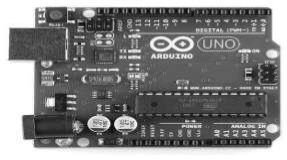
\includegraphics{arduiono-uno}}
        \caption{Example of a figure caption.}
        \label{fig}
    \end{figure}

    Figure Labels: Use 8 point Times New Roman for Figure labels. Use words
    rather than symbols or abbreviations when writing Figure axis labels to
    avoid confusing the reader. As an example, write the quantity
    ``Magnetization'', or ``Magnetization, M'', not just ``M''. If including
    units in the label, present them within parentheses. Do not label axes only
    with units. In the example, write ``Magnetization (A/m)'' or ``Magnetization
    \{A[m(1)]\}'', not just ``A/m''. Do not label axes with a ratio of
    quantities and units. For example, write ``Temperature (K)'', not
    ``Temperature/K''.

    \section*{Acknowledgment}

    The preferred spelling of the word ``acknowledgment'' in America is without
    an ``e'' after the ``g''. Avoid the stilted expression ``one of us (R. B.
    G.) thanks $\ldots$''. Instead, try ``R. B. G. thanks$\ldots$''. Put sponsor
    acknowledgments in the unnumbered footnote on the first page.


    \begin{thebibliography}{00}
        \bibitem{b1} S. Kaplan and C. G. Prato, “Risk factors associated with bus accident severity in the United States: a generalized ordered logit model,” Journal of Safety
        Research, vol. 43, no. 3, pp. 171–180, 2012.
        \bibitem{b2} RANGA SREEDHAR GALLA Diminishing Road Accidents On Sharp Curves Using Arduino Volume 1 Issue 5, November 2017.
        \bibitem{b3} Jessen Joseph Leo., R. Monisha.,et.al. : Vehicle movement control and accident avoidance in hilly track, IEEE Int. Conf. on Electronics and Communication
        Systems (ICECS).pp. 1-5(2014).
        \bibitem{b4} DEEKSHA ASHUTHA K. ARAVINDA B, CHAITHRA LAKSHMI C. Sensor based accident prevention system. International Journal of Computer
        Applications, pages 36–39, 2012.
        \end{thebibliography}

\end{document}

